% Proposal Skripsi
% Muhammad Ghazali - 0606036
\documentclass[a4paper, 12pt]{report}
\usepackage{setspace}
\usepackage{graphicx, times}
\usepackage[bahasa]{babel}
\usepackage{tikz}
\usepackage{gantt}
\usepackage{tabularx}
\usepackage[top=3cm, bottom=3cm, left=4cm, right=3cm]{geometry}

\selectlanguage{bahasa}
%Gummi|063|=)
\title{\textbf{Membangun Web API dengan menggunakan JSON sebagai format serialisasi data}}
\author{
Muhammad Ghazali\\
Program Studi Teknik Informatika\\
Fakultas Teknik\\
Universitas Widyatama
\\\texttt{<muhammad.ghazali@widyatama.ac.id>}
}
\date{\today}


\usepackage{graphicx}
\begin{document}

\maketitle

\onehalfspacing
\tableofcontents
\setcounter{tocdepth}{3}

\addcontentsline{toc}{chapter}{\listfigurename}
\listoffigures

\addcontentsline{toc}{chapter}{\listtablename}
\listoftables

% most research papers have an abstract, then there is a predefined commands
% for telling LaTeX which part of the content makes up the abstract. This
% should appear in its logical order, therefore, after the top matter, but
% before the main sections of the body.
\begin{abstract}
\onehalfspacing LayangLayang Mobile (LLM) merupakan salah perusahaan yang bergerak di bidang \textit{mobile application development}. Saat ini LayangLayang Mobile sedang mengembangkan sebuah produk bernama CampusLife. Produk yang dikembangkan tersebut merupakan aplikasi \textit{mobile} yang bertujuan untuk membantu civitas kampus mengakses informasi relevan tentang kampus mereka.

\onehalfspacing Setiap informasi yang ditampilkan melalui aplikasi \textit{mobile} CampusLife merupakan data yang sudah diolah dan diambil dari Web API\footnote{http://en.wikipedia.org/wiki/Web\_API} CampusLife. Saat ini LLM belum memiliki Web API tersebut. Berdasarkan kondisi tersebut, penulis bekerjasama dengan LLM untuk membangun Web API CampusLife. Web API yang akan dibangun bertujuan untuk membuka akses secara tidak langsung ke \textit{data store}\footnote{http://en.wikipedia.org/wiki/Data\_store} yang tersimpan di salah satu layanan \textit{Database as a Service}\footnote{http://en.wikipedia.org/wiki/Cloud\_database} yang digunakan oleh LLM di AppFog\footnote{http://www.appfog.com/}. Seluruh data-data \textit{event} yang tersimpan di \textit{data store} akan diolah oleh Web API menjadi data dengan format yang dapat dikonsumsi dengan mudah oleh aplikasi \textit{mobile} CampusLife. Proses pengelohan tersebut dinamakan serialisasi data\footnote{Lihat bagian Landasan teori: Serialiasi Data}.

\onehalfspacing Dalam penelitian ini penulis akan memilih format serialisasi data JSON untuk digunakan merepresentasikan setiap data-data \textit{event} dalam format yang dapat dikonsumsi oleh aplikasi \textit{mobile} CampusLife. Penulis memilih format serialisasi data JSON karena JSON lebih mudah dibaca ditulis dan dibaca oleh mesin (komputer) dan manusia. Selain itu JSON lebih mudah untuk diproses karena memiliki struktur yang lebih sederhana dibandingkan XML\cite{json-fat-free}\cite{json-vs-xml-debate}.

\begin{flushleft}
\onehalfspacing Kata kunci: Web API, JSON, Format Serialisasi Data
\end{flushleft}

\end{abstract}

% isi latar belakang dan masalah dibuat dengan mengikuti panduan:
% http://romisatriawahono.net/2012/06/18/kiat-menyusun-alur-latar-belakang-masalah-penelitian/
\chapter{Pendahuluan}
\section{Latar Belakang dan Masalah}
% menjelaskan obyek penelitian
\onehalfspacing CampusLife adalah \textit{mobile information directory application} yang dikembangkan oleh LayangLayang Mobile (LLM) untuk menyediakan informasi yang relevan kepada civitas kampus. Salah satu fitur utama yang akan dirilis dalam waktu dekat adalah menyediakan informasi \textit{event}-\textit{event} terbaru kepada civitas kampus. 

\onehalfspacing Setiap informasi yang ditampilkan melalui aplikasi \textit{mobile} CampusLife merupakan data yang sudah diolah dan diambil dari Web API\footnote{http://en.wikipedia.org/wiki/Web\_API} CampusLife. Saat ini LLM belum memiliki Web API dan penulis berniat untuk membangun Web API tersebut. Web API yang akan dibangun bertujuan untuk membuka akses secara tidak langsung ke \textit{data store}\footnote{http://en.wikipedia.org/wiki/Data\_store} yang tersimpan di salah satu layanan \textit{Database as a Service}\footnote{http://en.wikipedia.org/wiki/Cloud\_database} yang digunakan oleh LLM di AppFog\footnote{http://www.appfog.com/}. Seluruh data-data \textit{event} yang tersimpan di \textit{data store} akan diolah oleh Web API menjadi data dengan format yang dapat dikonsumsi dengan mudah oleh aplikasi \textit{mobile} CampusLife. Proses pengolahan tersebut dinamakan serialisasi data\footnote{Lihat bagian Landasan teori: Serialiasi Data}.

\onehalfspacing Di antara format serialisasi data yang sudah disebutkan di atas, XML\footnote{http://www.w3.org/XML/} dan JSON\footnote{http://json.org/} merupakan format serialisasi data yang paling terkenal saat ini\cite{comparison-of-data-serialization-formats}. Dalam penelitian ini penulis akan memilih format serialisasi data JSON untuk digunakan merepresentasikan setiap data-data \textit{event} dalam format yang dapat dikonsumsi oleh aplikasi \textit{mobile} CampusLife. Penulis memilih format serialisasi data JSON karena JSON lebih mudah dibaca ditulis dan dibaca oleh mesin (komputer) dan manusia. Selain itu JSON lebih mudah untuk diproses karena memiliki struktur yang lebih sederhana dibandingkan XML\cite{json-fat-free}\cite{json-vs-xml-debate}.

% menjelaskan rangkuman penelitian
\onehalfspacing \textit{Smartphone} sebagai perangkat tempat aplikasi \textit{mobile} CampusLife berjalan, merupakan salah satu \textit{mobile computing devices} yang memiliki masa hidup baterai dan ketersediaan \textit{bandwidth} yang terbatas.\cite{challenging-issues-and-limitations-of-mobile-computing}. Dengan kedua keterbatasan tersebut, dalam penelitian ini penulis akan mengkaji penerapan format serialisasi data JSON yang efektif untuk menghasilkan ukuran data yang optimal saat pengiriman data berlangsung dari Web API ke aplikasi \textit{mobile} CampusLife. Hasil akhir yang diharapkan adalah format serialisasi data JSON mampu menghasilkan ukuran data yang optimal untuk dikonsumsi oleh aplikasi \textit{mobile}.

% Pada bagian ini jelaskan rumusan masalah yang akan diteliti
\newpage
\section{Rumusan Masalah}
\onehalfspacing Berdasarkan latar belakang masalah yang telah dipaparkan, maka masalah yang akan diteliti dalam penelitian ini dapat dirumuskan sebagai berikut:
\begin{enumerate}
  \item Bagaimana membangun Web API dengan efektif agar data yang dikirimkan dapat memiliki ukuran data yang optimal untuk dikonsumsi oleh aplikasi \textit{mobile} CampusLife?
  \item Bagaimana JSON dapat diterapkan secara efektif agar data yang dihasilkan dapat memiliki ukuran data yang optimal untuk dikonsumsi oleh aplikasi \textit{mobile} CampusLife?
\end{enumerate}

% Tujuan dan manfaat penelitian
\section{Tujuan dan Manfaat Penelitian}
\onehalfspacing Tujuan dari pelaksanaan penelitian tugas akhir yang dilakukan penulis adalah:
\begin{enumerate}
  \item Membangun purwa-rupa Web API yang mampu mengirimkan data dengan ukuran data yang optimal untuk dikonsumsi oleh aplikasi \textit{mobile} CampusLife.
  \item Menerapkan JSON dengan efektif untuk menghasilkan data dengan ukuran data yang optimal untuk dikonsumsi oleh aplikasi \textit{mobile} CampusLife.
\end{enumerate}

\onehalfspacing Penulis mengharapkan hasil penelitian ini akan membawa manfaat positif bagi kepentingan dunia akademik dan praktis dalam hal penerapan format serialisasi data JSON untuk menghasilkan ukuran data yang optimal untuk dikonsumsi oleh aplikasi \textit{mobile}.

\section{Batasan Masalah}
\onehalfspacing Untuk memperjelas ruang lingkup pelaksanaan penelitian, penulis memiliki batasan masalah meliputi:
\onehalfspacing
\begin{enumerate}
  \item Pembangunan Web API hanya akan sampai pada tahap purwa-rupa.
  \item Pembangunan Web API hanya akan meliputi API untuk mengambil data-data \textit{event}.
  \item JSON hanya mampu merepresentasikan data dalam bentuk teks, oleh karena itu data yang akan digunakan hanya terbatas pada data yang berbasis teks.
  \item Skema data \textit{event} akan disediakan oleh pihak LLM.
  \item Penulis akan melakukan demo untuk mengakses Web API melalui Android\footnote{http://www.android.com/} \textit{smartphone} yang sudah terpasang aplikasi mobile CampusLife. Aktivitas demo akan difokuskan pada pengambilan  data-data \textit{event} dari purwa-rupa Web API yang dibuat oleh penulis.
  \item Tidak membahas mengenai keamanan perangkat lunak, data dan jaringan.
  \item Pengembangan perangkat lunak menggunakan sebagian praktek dari \textit{Agile} dan tidak akan membahas \textit{Agile} secara komprehensif.
\end{enumerate}

\section{Metodologi Penelitian}
\onehalfspacing Adapun tahapan penelitian yang akan dilakukan oleh penulis tahap-tahap berikut:
\begin{enumerate}
  \item Identifikasi masalah. Pada tahap ini penulis merumuskan masalah yang akan diteliti.
  \item Perumusan hipotesis. Pada tahap ini penulis merumuskan jawaban sementara dari permasalahan yang diteliti.
  \item Pengujian hipotesis. Pada tahap ini penulis menguji penerapan JSON terhadap Web API yang sudah dibangun dan pembangunan perangkat lunak akan dilakukan dengan menggunakan metodologi pengembangkan perangkat lunak \textit{Agile}. 
  \item Kesimpulan. Pada tahap ini penulis menganalisa hasil pengujian hipotesis.
\end{enumerate}

\onehalfspacing Adapun cara untuk menunjang penelitian dilakukan dengan melakukan studi kepustakaan, yaitu pengumpulan data dari artikel-artikel, jurnal dan buku-buku yang berhubungan dengan topik pembahasan di penelitian.

% sistematika penulisan
\section{Sistematika Penulisan}
Sistematika pembahasan laporan ini terdiri dari enam bab, yaitu:
\begin{description}
  \item[Bab I Pendahuluan] Pada bagian ini berisikan pendahuluan laporan yang berisi latar belakang, rumusan masalah, tujuan dan manfaat penelitian, batasan masalah, metode penelitian dan sistematika penulisan laporan.
  \item[Bab II Landasan Teori] Pada bagian ini akan dibahas landasan teori yang berkaitan dan digunakan selama masa penelitian.
  \item[Bab III Analisis Sistem] Pada bagian ini akan dibahas hasil analisis terhadap masalah.
  \item[Bab IV Desain Sistem] Pada bagian ini akan dibahas hasil perancangan sistem.
  \item[Bab V Implementasi dan Pengujian Sistem] Pada bagian ini akan dibahas proses implementasi dan pengujian sistem berdasarkan kriteria pengujian yang sudah ditentukan.
  \item[Bab VI Penutup] Pada bagian ini berisikan kesimpulan dan saran yang didapatkan dari hasil penelitian.
\end{description}

\chapter{Landasan Teori}
% TODO Penjelasan tentang high-level architecture CampusLife dipindahkan ke bab 3
\section{High-level Architecture CampusLife}
\onehalfspacing Secara umum CampusLife dibangun dengan menggunakan \textit{three-tier architecture} yang terdiri dari 3 tingkat, yaitu \textit{presentation}, \textit{logic} dan \textit{data}. CampusLife dibangun dengan menggunakan \textit{three-tier architecture} dengan tujuan agar pengembang aplikasi bisa melakukan perubahan dengan relatif mudah. Berikut adalah gambaran visual dari arsitektur CampusLife:
\begin{figure}[htp]
\centering
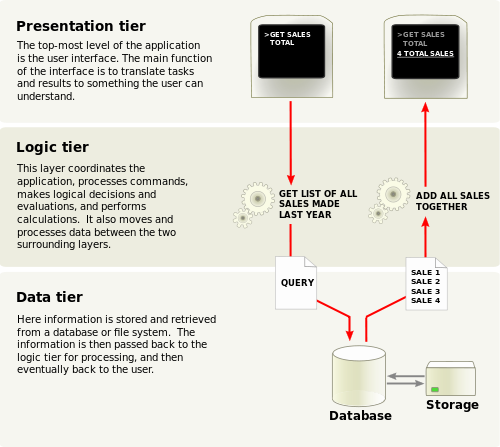
\includegraphics[scale=0.40]{images/test.png}
\caption{High-level architecture CampusLife}
\label{High-level architecture CampusLife}
\end{figure}

\subsection{Presentation Tier}
\onehalfspacing \textit{Presentation tier} adalah \textit{tier} paling atas dari aplikasi CampusLife. \textit{Tier} ini menampilkan informasi terkait dengan layanan seperti menampilkan daftar event dan menampilkan daftar pengunjung event kepada pengguna melalui \textit{mobile application}. Layanan informasi seperti ini akan disediakan melalui Web API yang berada di \textit{logic tier} dan dapat diakses melalui \textit{client} seperti \textit{mobile application} dan \textit{browser}. Secara sederhana \textit{presentation tier} adalah tingkat dimana pengguna dapat mengakses aplikasi secara langsung. Dalam konteks pengerjaan penelitian tugas akhir ini, \textit{mobile application} CampusLife akan berada di \textit{tier} ini\cite{multitier-architecture-wikipedia}.

\subsection{Logic Tier}
\onehalfspacing \textit{Logic tier} adalah \textit{tier} yang berfungsi untuk mengontrol fungsionalitas aplikasi dengan melakukan pengolahan rinci. Contoh pengolahan rinci yang bisa dilakukan di \textit{tier} ini adalah mengambil daftar event. Dalam konteks pengerjaan penelitian tugas akhir ini, Web API akan berada di \textit{tier} ini\cite{multitier-architecture-wikipedia}.

\subsection{Data Tier}
\onehalfspacing \textit{Data tier} adalah \textit{tier} yang terdiri dari satu atau lebih \textit{server} basis data. Disini setiap informasi disimpan dan diambil. \textit{Tier} ini akan menjaga data tetap netral dan indenpenden dari \textit{application server} atau \textit{business logic}. Selain itu dengan memberikan data di \textit{tier} sendiri akan meningkatkan \textit{scalability} dan \textit{performance}. Dalam konteks pengerjaan penelitian tugas akhir ini, penulis menggunakan MongoDB sebagai basis data di \textit{tier} ini\cite{multitier-architecture-wikipedia}.

\subsection{Keuntungan dari Arsitektur Three-tier}
\onehalfspacing CampusLife dibangun dengan menggunakan arsitektur three-tier untuk mendapatkan beberapa keuntungan berikut:

\begin{enumerate}
  \item Lebih mudah untuk memodifikasi atau mengganti \textit{tier} apapun tanpa mempengaruhi \textit{tier} lainnya.
  \item Memisahkan aplikasi dan fungsi database berarti \textit{load balancing} yang lebih baik.
\end{enumerate}

\section{Web API}
\onehalfspacing
\subsection{Apa itu Web API}
\textit{Application programming interface} (API) adalah sebuah protokol yang dimaksudkan untuk digunakan sebagai antarmuka oleh komponen perangkat lunak untuk berkomunikasi satu sama lain. Ketika digunakan dalam konteks pengembangan \textit{web}, API biasanya didefinsikan sebagai satu set \textit{Hypertext Transfer Protocol} (HTTP) \textit{request message}, dan disertai dengan \textit{response message} dalam \textit{Extensible Markup Language} atau \textit{JavaScript Object Notation}.

\onehalfspacing Praktek penerbitan Web API telah memungkinkan masyarakat \textit{web} seperti pengembang aplikasi berbasis \textit{web} untuk membuat arsitektur terbuka untuk berbagi konten dan data antara masyarakat dan aplikasi. Dengan cara ini, konten yang dibuat dalam satu tempat dapat dikirimkan secara dinamis dan diperbaharui di beberapa lokasi di \textit{web} \cite{api-wikipedia}.

\subsection{Kenapa Web API}
Ketika Anda menjalankan aplikasi \textit{web}, pada saat tertentu Anda ingin menyediakan Web API. Berikut adalah berapa alasan yang umum kenapa perlu menyediakan Web API \cite{apis-linux-journal}:

\begin{enumerate}
  \item Untuk memungkinkan pengguna Anda mengakses data mereka melalui aplikasi pihak ketiga. Pertimbangkan berapa banyak pihak ketiga Twitter klien yang ada\footnote{http://en.wikipedia.org/wiki/List\_of\_Twitter\_services\_and\_applications}, semua menggunakan API Twitter, daripada mengakses langsung ke situs \textit{web}. Hal yang sama berlaku untuk Amazon\footnote{http://www.amazon.com/} dan eBay\footnote{http://www.ebay.com/}, antara lain, yang memungkinkan pengguna untuk mengakses data katalog mereka dan bahkan mengeksekusi penjualan, semua melalui API.
  \item Untuk memungkinkan pengembang aplikasi mobile untuk mengakses situs Anda dengan mengirim dan mengambil data menggunakan HTTP.
  \item Untuk memungkinkan aplikasi Anda sendiri untuk mengakses data sendiri melalui panggilan Ajax\footnote{https://developer.mozilla.org/en/docs/AJAX}. Bila Anda membuat panggilan JavaScript di latar belakang menggunakan Ajax, kemungkinan besar Anda akan ingin menggunakan panggilan API, menerima XML atau JSON, bukan HTML yang membutuhkan \textit{parsing} lebih lanjut.
\end{enumerate}

\subsection{RESTful Web API}
\onehalfspacing \textit{Representational State Transfer} (REST) mendefinisikan seperangkat prinsip arsitektur dimana penulis dapat merancang layanan Web yang berfokus pada sistem \textit{resource}, termasuk bagaimana keadaan \textit{resource} dipanggil dan ditransfer melalui HTTP oleh berbagai macam klien yang ditulis dalam bahasa (pemrograman) yang berbeda. Jika diukur dengan jumlah layanan Web yang menggunakannya, REST telah muncul dalam beberapa tahun terakhir sebagai model desain layanan Web yang dominan. Bahkan, REST memiliki dampak besar di Web yang telah sebagian besar menggantikan desain antarmuka berbasis SOAP-WSDL dan karena REST memiliki gaya yang jauh lebih sederhana untuk digunakan \cite{ws-restful}.

\onehalfspacing RESTful Web API (juga disebut \textit{RESTful web service}) adalah Web API yang diimplementasikan dengan menggunakan HTTP dan prinsip-prinsip REST\footnote{Architectural Styles and
the Design of Network-based Software Architectures http://www.ics.uci.edu/~fielding/pubs/dissertation/top.htm}.

% Daftar buku atau karangan yang merupakan sumber rujukan dari sebuah
% tulisan atau karangan atau daftar tt suatu subjek ilmu, daftar pustaka
% Jumlah maksimal daftar pustaka dan referensi yang bisa dimasukkan adalah 100 item
\begin{thebibliography}{99}
\singlespacing 

% use the surname of the first author, followed by the last two digits of
% the year (hence lamport94)

\bibitem{challenging-issues-and-limitations-of-mobile-computing}
Deepak, G., and Dr. Pradeep B S. "Challenging Issues and Limitations of Mobile Computing."
  \emph{International Journal of Computer Technology and Applications} 3.1 (2012): Academic Journals Database. Web. 8 Jan. 2013.
  
  \bibitem {comparison-of-data-serialization-formats}
Audie Sumaray dan S. Kami Makki. "A comparison of data serialization formats for optimal efficiency on a mobile platform". \emph{6th International Conference on Ubiquitous Information Management and Communication} (2012): Artikel No. 48. ACM Digital Library. Web. 24 Jan 2013.
  
\bibitem{json-vs-xml-debate}
  \emph{Debate: JSON vs. XML as a data interchange format}
  http://www.infoq.com/news/2006/12/json-vs-xml-debate
  diakses pada 20 Januari 2012.
  
\bibitem{serialization-wikipedia}
  \emph{Serialization}
  http://en.wikipedia.org/wiki/Serialization
  diakses pada 24 Januari 2012.
  
\bibitem{agile-wikipedia}
  \emph{Agile software development}
  http://en.wikipedia.org/wiki/Agile\_software\_development
  diakses pada 24 Januari 2012.
  
\bibitem{json-fat-free}
  \emph{JSON: The Fat-Free Alternative to XML}
  http://www.json.org/xml.html
  diakses pada 20 Januari 2012.
  
\bibitem{multitier-architecture-wikipedia}
  \emph{Wikipedia: Multitier architecture}
  http://en.wikipedia.org/wiki/Multitier\_architecture
  diakses pada 15 Maret 2013.
  
\bibitem{three-tier-architecture}
  \emph{Three-Tier Architecture}
  http://www.linuxjournal.com/article/3508
  diakses pada 18 Maret 2013.
  
\bibitem{api-wikipedia}
  \emph{Application Programming Interface}
  http://en.wikipedia.org/wiki/Application\_programming\_interface
  diakses pada 22 Maret 2013.
  
\bibitem{web-api}
  \emph{Web API}
  http://en.wikipedia.org/wiki/Web\_API
  diakses pada 20 Januari 2013.
  
\bibitem{apis-linux-journal}
  \emph{APIs}
  http://www.linuxjournal.com/content/apis
  diakses pada 20 Januari 2013.

\bibitem{ws-restful}
  \emph{RESTful Web services: The basics}
  \\http://www.ibm.com/developerworks/webservices/library/ws-restful/
  diakses pada 14 September 2012.

\bibitem{introducing-json}
  \emph{Introducing JSON} http://www.json.org/
  diakses pada 20 Januari 2013.
    
\bibitem{rest-soap}
  \emph{How REST replaced SOAP on the Web: What it means to you}
  http://www.infoq.com/articles/rest-soap
  diakses pada 14 September 2012.
 
\end{thebibliography}

\end{document}

